\documentclass[aspectratio=169]{beamer}
\usepackage[utf8]{inputenc}
\usepackage{tikz}
\usepackage{tikz-cd}
\usepackage{tikz-layers}
\usepackage{pifont}
\usepackage{pgfpages}
\usepackage{pgfplots}
\usepackage{graphicx}
\usepackage[export]{adjustbox}
\usepackage{qrcode}
\usepackage{caption}
\usepackage{minted}
\usepackage[svgnames]{xcolor}
\usetikzlibrary{backgrounds}
\usetikzlibrary{decorations.pathreplacing}

% the drgtheme files live once at the repo root, in ../../theme/
\makeatletter
\def\input@path{{../../theme/}}
\makeatother
\graphicspath{{../images/}{../../theme/}}

\usetheme{drgtheme}

%setup cover page variables
\title{Control System: Phases 0 and 1}
\author{
    Dr Max Champneys
}
\institute[UoS]{
    School of Mechanical, Aerospace, and Civil Engineering,\\
    University of Sheffield, UK
}
\date{MAC 233: \hspace{0.1em}\textbf{11/11/2026}}
%setup footer variables
\runninginstitute{MAC 233, School of MAC, University of Sheffield}
\email{max.champneys@sheffield.ac.uk}

%Begin Document
\begin{document}

%Create Title Page
\maketitle

\begin{frame}{MAC 233: Labs Overview}
    \begin{center}
        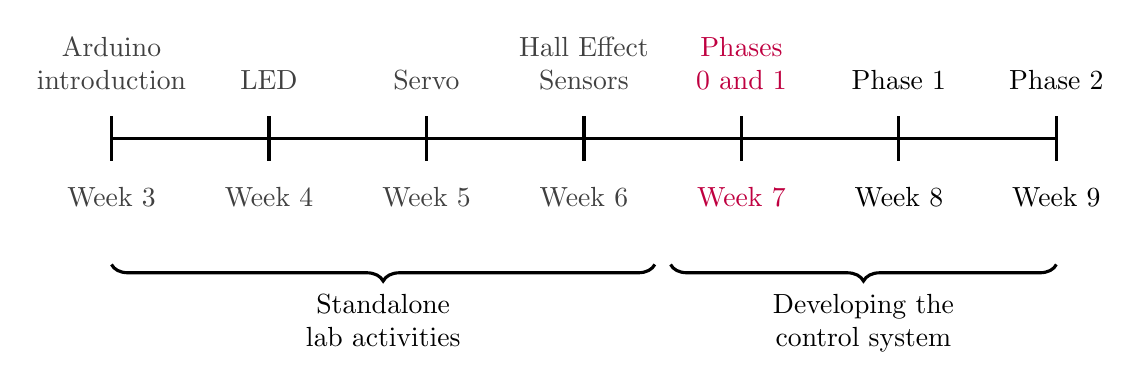
\begin{tikzpicture}[
            timeline/.style={color=black, line width=0.4mm},
            pastnode/.style={align=center, color=darkgray},
            currentnode/.style={align=center, color=purple},
            futurenode/.style={align=center, color=black}
        ]
            %line
            \draw[timeline] (-6, 0) -- (6, 0);

            % week ticks
            \foreach \x in {-6, -4, -2, 0, 2, 4, 6}{
                \draw[timeline] (\x, -0.28) -- (\x, 0.28);
            }

            % weeks (below the line)
            \node[pastnode, below] at (-6, -0.5) {Week 3};
            \node[pastnode, below] at (-4, -0.5) {Week 4};
            \node[pastnode, below] at (-2, -0.5) {Week 5};
            \node[pastnode, below] at (0, -0.5) {Week 6};
            \node[currentnode, below] at (2, -0.5) {Week 7};
            \node[futurenode, below] at (4, -0.5) {Week 8};
            \node[futurenode, below] at (6, -0.5) {Week 9};

            % activities (above the line)
            \node[pastnode, above] at (-6, 0.5) {Arduino\\introduction};
            \node[pastnode, above] at (-4, 0.5) {LED};
            \node[pastnode, above] at (-2, 0.5) {Servo};
            \node[pastnode, above] at (0, 0.5) {Hall Effect\\Sensors};
            \node[currentnode, above] at (2, 0.5) {Phases\\0 and 1};
            \node[futurenode, above] at (4, 0.5) {Phase 1};
            \node[futurenode, above] at (6, 0.5) {Phase 2};

            % phases
            \draw[timeline, decorate, decoration={brace, amplitude=6pt, mirror}] (-6, -1.6) -- (0.9, -1.6);
            \node[futurenode, below] at (-2.55, -1.85) {Standalone\\lab activities};
            \draw[timeline, decorate, decoration={brace, amplitude=6pt, mirror}] (1.1, -1.6) -- (6, -1.6);
            \node[futurenode, below] at (3.55, -1.85) {Developing the \\ control system};

        \end{tikzpicture}
    \end{center}
\end{frame}

\begin{frame}{The next three weeks}
    \large
    \begin{center}
        \begin{tabular}{lll}
            \textbf{Week} & \textbf{Phase} & \textbf{Mini rig?} \\
            \hline
            7 & 0: how the control system works & No \\
              & 1: build steps 1--3 & No, use a magnet \\
            8 & 1: build steps 4--5 & Only for step 5 \\
            9 & 2: developing the control system & Yes \\
        \end{tabular}
    \end{center}
    \vspace{1em}
    Your rig isn't finished? That's fine: steps 1--4 only need your Arduino kit and a magnet.
\end{frame}

\begin{frame}{The mini rig}
    \begin{center}
        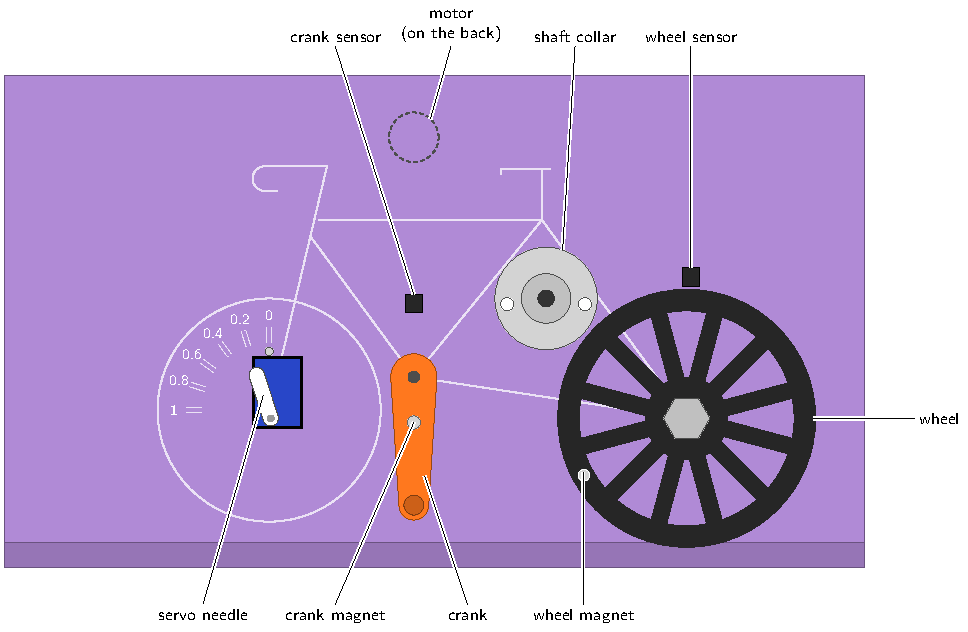
\includegraphics[height=.75\textheight]{mini-rig.pdf}
    \end{center}
\end{frame}

\begin{frame}{The control system}
    \begin{center}
        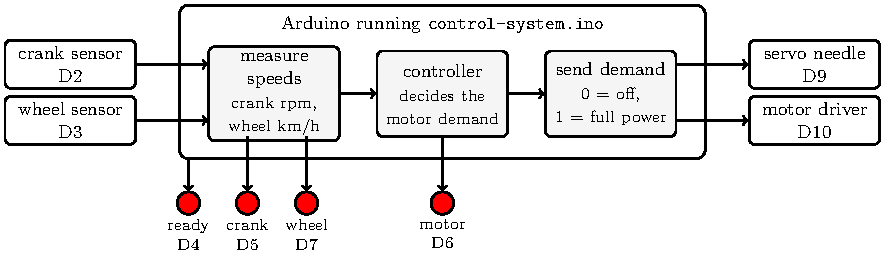
\includegraphics[width=\textwidth]{block-diagram.pdf}
    \end{center}
    \vspace{.5em}
    Only help while the rider is pedalling, and never above 25\,km/h.
\end{frame}

\begin{frame}{Building it: one part at a time}
    \Large
    Build everything, then test it: if it doesn't work, where is the fault?

    \vspace{.75em}
    Build one part, then test it: the fault is in what you just added.
    \vspace{1.5em}
    \begin{center}
        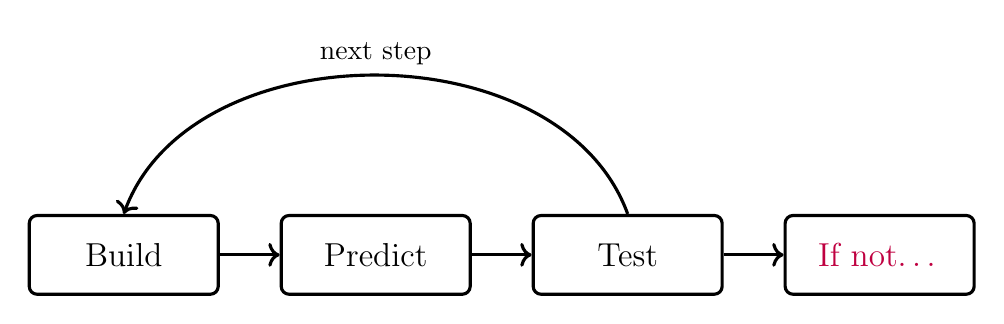
\begin{tikzpicture}[
            stage/.style={draw, line width=.4mm, rounded corners=1mm,
                minimum width=2.4cm, minimum height=1cm, font=\large},
            arrow/.style={->, line width=.4mm},
        ]
            \node[stage] (build) at (0, 0) {Build};
            \node[stage] (predict) at (3.2, 0) {Predict};
            \node[stage] (test) at (6.4, 0) {Test};
            \node[stage, text=purple] (ifnot) at (9.6, 0) {If not\ldots};
            \draw[arrow] (build) -- (predict);
            \draw[arrow] (predict) -- (test);
            \draw[arrow] (test) -- (ifnot);
            \draw[arrow] (test.north) to[out=110, in=70] node[above, font=\normalsize]
                {next step} (build.north);
        \end{tikzpicture}
    \end{center}
\end{frame}

\begin{frame}{Today}
    \Large
    \textbf{Phase 0}: read through the sketch, then answer the check questions with a partner.

    \vspace{1em}
    \textbf{Phase 1}: build steps 1--3 on the bench. Pass the magnet by hand to test the sensors.

    \vspace{1em}
    Upload the sketch once, at the start of step 1. You won't change it until Phase 2.
\end{frame}

\begin{frame}{Help}
    \normalsize
    \begin{columns}
        \begin{column}{.33\textwidth}
            \begin{center}
                \textbf{Worksheet}\\
                \vspace{.5em}
                \qrcode[hyperlink, height=3cm]{https://github.com/MDCHAMP/MAC233/blob/main/control-system/docs/control-system.pdf}
            \end{center}
        \end{column}
        \begin{column}{.33\textwidth}
            \begin{center}
                \textbf{Sketch}\\
                \vspace{.5em}
                \qrcode[hyperlink, height=3cm]{https://github.com/MDCHAMP/MAC233/blob/main/control-system/control-system.ino}
            \end{center}
        \end{column}
        \begin{column}{.33\textwidth}
            \begin{center}
                \textbf{Nano Every pinout}\\
                \vspace{.5em}
                \qrcode[hyperlink, height=3cm]{https://docs.arduino.cc/resources/pinouts/ABX00028-full-pinout.pdf}
            \end{center}
        \end{column}
    \end{columns}

    \vspace{3.5em}
    Problems? Raise your hand and someone will come and help you.
\end{frame}

\end{document}
